\chapter{}

Um Die Folgenden Sachverhalte leichter einsehen zu können macht es Sinn,
sich zuerst schon bekannte Objekte/Dinge/Sachverhalte vor Augen zu führen.
\begin{figure}[h!]
 \centering
    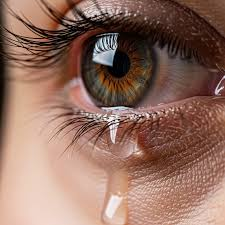
\includegraphics[width=0.3\textwidth]{pictures/Auge.jpeg}
    \caption{\url{https://creativecommons.org/licenses/by-nd/4.0/}}
 \end{figure}

In diesem Fall macht es vor allem Sinn, Folgen zu betrachten.
Sei also $\alpha$ eine Abbildung von $\mathbb{B} \to X$ 
also die Folge $\alpha(0), \alpha(1), \alpha(2), \dots \alpha(n), \dots $
Weiters betrachte die Abbildung $\beta: \mathbb{N} \to X$
wobei wir $\beta$ als Teilfolge von $\alpha$ bezeichnen. Wenn es eine streng
monoton wachsende Abbildung $k: \mathbb{N} \to \mathbb{N}$ gibt, so dass
$\beta(n) = \alpha(k(n))$ für alle $n \in \mathbb{N}$ gilt.

$$
\begin{tikzcd}
\mathbb{N} \arrow[r, "\alpha"]  & X \\
\mathbb{N} \arrow[ur, "\beta"'] \arrow["\kappa", u] &
\end{tikzcd}
$$

$$
\text{mit } \quad \beta = \alpha \circ \kappa
$$

\dfn{Teilnetz}
{
Sind $(I, \preceq_I)$ und $(J, \preceq_J)$ zwei gerichtete Mengen,
ist $X$ eine Menge und $\alpha : I \to X$ ein Netz in $X$, 
Und $\kappa : J \to I$ eine Funktion, so dass
 
$$
\bigstar
\forall i_0 \in I \; \exists j_0 \in J : \; \forall j \succeq_J j_0
\Rightarrow \kappa(j) \succeq_I i .
$$
Dann ist $\alpha \circ \kappa : J \to X$ ein \textbf{Teilnetz} von $\alpha$.
Ist $(J, \preceq_J) = (\mathbb{N}, \leq)$, 
dann wäre $\alpha \circ \kappa : J \to X$ Eine \textbf{Teilfolge}.
}
\nt
{ 
    Seien $\langle I, \preceq_I \rangle$ und $\langle J, \preceq_J \rangle$ 
    gerichtete Mengen und $\kappa : J \to I$ eine monotine Abbildung.
    wenn 
    \begin{itemize}
        \item $\kappa$ monoton
        \item $\forall i \in I \exists j_0 \in J: \kappa(j_0) \succeq_I i$
    \end{itemize}
    dann ist $\alpha \circ \kappa(j) $ ein Teilnetz von $\alpha$.

    \begin{proof}{Beweis der Implikation:}\\
        Sei $i_0 \in I$ beliebig. Dann gibt es ein $j_0 \in J$ mit 
        $\kappa(j_0) \succeq_I i_0$. Für alle $j \succeq_J j_0$ gilt
        $\kappa(j) \succeq_I \kappa(j_0) \succeq_I i_0$.
    \end{proof}
}

Das soll \emph{nicht} zur verwirrung führen. Aber:\\
Der implikationspfeil ist in disem Fall nicht nur eine Stylistische entscheidung.
und wir erfahrne später das es sich eigentlich um eine aquivalenz handelt. 
Es handlet sich also wirklich nur um eine Implikation (dh. die andere richtung
gilt nicht) 
In der Mathematischen Literatur wird anstelle von unserer 
Definition von Teilnetzen
Die eigenscchaften der Bemerjung als Definition verwendet.

\thm{}
{
    ei $(X, \mathcal{T})$ topologischer Raum, $(I, \preceq_I)$ gerichtete Menge,  
$\varphi : I \to X$, Netz in $X$, $x \in X$.  

Dann sind äquivalent:

\begin{enumerate}
\item[(i)] $\varphi$ konvergiert gegen $x$.
\item[(ii)] Jedes Teilnetz von $\varphi$ konvergiert gegen $x$.
\item[(iii)] Jedes Teilnetz von $\varphi$ hat ein Teilnetz, das gegen $x$ konvergiert.
\end{enumerate}
}

\begin{proof}{Satz: 4.0.2:}\\
    \begin{itemize}
        \item[ (i) $\Rightarrow$ (ii)]
        Sei $\langle J, \preceq_J \rangle$ und$\kappa : J \to I$ 
        ein Teilnetz von $\varphi$ also erfüllt $\bigstar$.\\
        Sei $U \in \mathscr{text}{U}(x)$
        Wähle $i_0 \in I$ so dass $\forall i \succeq_I i_0 : \varphi(i) \in U$
        Nach $\bigstar$ gibt es ein $j_0 \in J$ so dass 
        $\forall j \succeq_J j_0 : \kappa(j) \succeq_I i_0$.
        Also gilt für alle $j \succeq_J j_0$:
        $$\varphi(\kappa(j)) \in U
        $$
        Also konvergiert das Teilnetz gegen $x$.
        \item[(ii) $\Rightarrow$ (iii)]
        Jedes Netz ist ein Teilnetz von sich selbst. 
        $I \overset{\text{id}}{\longrightarrow} I \overset{\text{id}}{\longrightarrow} X$ 
        Sei $\varphi \circ \kappa$ Teilnetz von 
        $\varphi \Rightarrow \varphi \circ \kappa$ konvergiert gegen 
        $x \Rightarrow \varphi \circ \operatorname{id}$ konvergiert gegen $x$.
        \item[(iii) $\Rightarrow$ (i)]
        Für diese richtung verwenden wir Kontraposition.
        - Weil wir das schon länger nicht gemaht haben -\\
        $\neg (i) \Rightarrow \neg (iii)$:\\
        Wähle $U \in \mathscr{U}(x)$ 
        $\forall i_0 \in I  \exists i \succeq i_0$
        sodass $\varphi(i) \notin U$ 
        $$
        (**)\quad J := \{ i \in I \mid \varphi(i) \notin U \} \subseteq I
        $$
        Diesmal ist es leichter, die Bemerkung zu verwenden\\
        Definiere $j_1, j_2 \in J : j_1 \preceq_J j_2 :\Leftrightarrow j_1 \preceq_I j_2$.\\
        - Die Einschränkung der Ordnung auf $I$ als Ordnung auf $J$ -\\
        Damit ist $(J, \preceq_J)$ reflexiv und transitiv.
\bigskip
        Seien $j_1, j_2 \in J$.
        Wähle $i \in I : j_1 \succeq_I i, j_2 \succeq i$.
        $\Rightarrow j_1 \succeq i, j_1 \succeq_J i, j_2 \succeq_J i$. 
        $\Rightarrow (J, \succeq_J)$ ist gerichtete Menge.

        Definiere:\\
        $$
        \kappa :
        \begin{cases}
        j \mapsto j \\
        i \mapsto i
        \end{cases}
        $$

        Sei $i \in I$.
        Wegen $(**)$ wähle $j_0 \in I$ 
        sodass $\varphi(j_0) \notin U$. 
        $j_0 \in J$.

        Sei $(K, \le_K)$ eine gerichtete Menge, mit 
        $\lambda : K \to J$ mit $(\bigstar)$.
        Also $(\varphi \circ \kappa) \circ \lambda : K \to X$.

        Angenommen 
        $$
        \lim_{k \in K} [(\varphi \circ \kappa) \circ \lambda](k) = x.
        $$

        Wähle $k_0 \in K : \forall k \succeq k_0 : [(\varphi \circ \kappa) \circ \lambda](k) \in U.$ \\
        Was ein Widerspruch ist, da $\varphi(\kappa(\lambda(k_0))) \notin U$
        Per definition von $(\varphi \circ \kappa) \circ \lambda$.

    \end{itemize}
\end{proof}

Wir sehen also im, vergleich zu Folgen haben wir keine Index schlacht
mehr. 
Dafür haben wir jetzt sehr vile abbildungen $\circ$ abbildungen.

\thm{}
{
    Sei $\langle X, \mathcal{T} \rangle$ ein topologischer Raum.
    \begin{itemize}
        \item[(i)] $A \subseteq X$ ist abgeschlossen $\Leftrightarrow$
        für jedes Netz $\varphi : I \to A \subseteq X$  in A, 
        das gegen $x \in X$ konvergiert, gilt $x \in A$.
        \item[(ii)] Sei $\langle Y, \mathcal{S} \rangle$ ein weiterer topologischer Raum.
        Eine Abbildung $f : X \to Y$ ist stetig $\Leftrightarrow$
        für jedes Netz $\alpha : I \to X$ in $X$, das gegen ein $x \in X$ konvergiert,
        gilt, 
        $$
        \lim_{i \in I} \alpha(i) 
        \leftarrow \lim_{i \in I} (f \circ \alpha)(i) = f(x)
        $$.
    \end{itemize}
}

Der zweite punkt ist so zu verstehen das wenn x eine grenzwert von $\alpha$ ist
dann ist $f(x)$ der grenzwert von $f \circ \alpha$
Der Grenzwert muss hir nicht eindeutig sein.

\begin{proof}{Satz: 4.03:}\\
    \begin{itemize}
        \item["(i)$\Rightarrow$"]
        Sei $A \subseteq X$ abgeschlossen, 
        angenommen $\alpha : I \to A$ ist ein Netz in $X$, mit $x \in X$.
        So dass $\lim_{i \in I} \alpha(i) = x$. und $x \notin A$.
        Sei $U := X \setminus A \in \mathcal{U}(x)$.
        aber $\forall i \in I : \alpha(i) \in A \Rightarrow \alpha(i) \notin U$.
        \item["(i)$\Leftarrow$"]
        Sei $A \subseteq X$ nicht abgeschlossen. 
        Dann ist $X \setminus A$ nicht offen. 
        Also gibt es ein $x \in X \setminus A$ so dass 
        $\forall U \in \mathcal{U}(x) : U \not\subseteq X \setminus A$.
        $\Rightarrow \forall U \in \mathscr{U}(x) : \neg (U \subset X \setminus A)$
        (dh.: $U \cap A \neq \emptyset$).
        Wähle $\alpha : \mathscr{U}(x) \to X$ mit $\alpha(U) \in U_1 $.
        Das können wir dank des Auswahlaxioms. So machen
        Für $U_1, U_2 \in \mathscr{U}(x)$ mit $U_1 \preceq U_2 : \Leftrightarrow U_1 \supseteq U_2$.
        Sei $\langle \mathscr{U}(x), \preceq \rangle$ eine gerichtete Menge.
        Also Transitivität und Reflexivität sind klar.
        Seien $U_1, U_2 \in \mathscr{U}(x)$.
        Wähle $U_3 \in \mathscr{U}(x)$ mit $U_3 \subseteq U_1 \cap U_2$.
        Dann ist $U_3 \preceq U_1$ und $U_3 \preceq U_2$.
        Also ist $\langle \mathscr{U}(x), \preceq \rangle$ eine gerichtete Menge.
        Sei $U \in \mathscr{U}(x)$.\\
        $\alpha$ ist konvergent gegen $x$.
        Sei $U \in \mathscr{U}(x)$. Setze $U_0 := U$.
        Sei $V \in \mathscr{U}(x)$ mit $V \preceq U_0$.
        Das heißt $V \subseteq U_0$.
        Also gilt $\alpha(V) \in V \subseteq U_0$.
        Damit haben wir ein netz in $A$ gefunden das gegen $x$ konvergiert.
        \item[(ii)"$\Leftarrow$"]
        Sei $\alpha : I \to A$ ein Netz in $X$ mit $\lim_{i \in I} \alpha(i) = x$.
        $A \subseteq \bar \{A\}$
        \item["(ii)$\Rightarrow$"]
        Sei $x \in  \bar{A} \Rightarrow 
        \forall U \in \mathcal{U}(x) : U \cap A \neq \emptyset$.
        \item["(i)$\Rightarrow$(ii)"]
        Sei $A \subseteq Y$ Abgeschlossen 
        Und $alpha : I \to f^{-1}(A)$, 
        mit $\lim_{i \in I} \alpha(i) = x$, $x \in X$.
        $\Rightarrow \lim_{i \in I} (f \circ f_\alpha)(i) = f(x)$
        Da $(f \circ f_\alpha)(i) \in A$ für alle $i \in I$, folgt  
        $f(x) \in \overline{A}$
        $\Rightarrow  x \in f^{-1}(A)$
        \end{itemize}
        
\end{proof}
